\documentclass[12pt,a4paper]{report}

\makeatletter

\def\author#1{\gdef\insertauthor{#1}\gdef\@author{#1}\hypersetup{pdfauthor={#1}}}
\def\title#1{\gdef\inserttitle{#1}\gdef\@title{#1}\hypersetup{pdftitle={#1}}}
\def\keywords#1{\gdef\insertkeywords{#1}\hypersetup{pdfkeywords={#1}}}
\def\subject#1{\gdef\insertsubject{#1}\hypersetup{pdfsubject={#1}}}

\makeatother

\RequirePackage[final,breaklinks,bookmarks]{hyperref}

\hypersetup{%
    colorlinks=true,
    allcolors=black,
    pdfcreator  = {\LaTeX\ with package \flqq hyperref\frqq},
    pdfproducer = {pdfeTeX-0.\the\pdftexversion\pdftexrevision}
}


%############################################################################
%########################### Change This ####################################
%############################################################################
%replace with German "Bachelor Thesis", "Master Thesis" or "Diplomarbeit" or
%replace with English "Bachelor's Thesis", "Master's Thesis"  
\subject{Master Thesis}
%put your title here
\title{Optimizing Agent Behavior and Minimizing User Cognitive Load for Mixed Human-Robot Teams}
%your name
\author{Christopher O'Hara}
% your matrikelnummer
\newcommand{\trmatrikelnummer}{406037}
%supervisor
\newcommand{\trbetreuerA}{Christopher-Eyk Hrabia}
%\newcommand{\trbetreuerA}{Dipl.-Inf. Christian Scheel}
%reviewer 1
\newcommand{\trguta}{Prof. Dr.-Ing. habil. Sahin Albayrak}
%reviewer two
\newcommand{\trgutb}{Prof. Dr. Odej Kao}
\date{\today}
%put some meaningful keywords, these are only examples
\keywords{Multi-Agent Systems, Machine Learning, Human-Robot Interaction}

%###################################################################################
%###################### Document Defintions ########################################
%###################################################################################
%aubrey: no real need to change these
%how to handle spaces
\sloppy
\makeindex

\usepackage[utf8]{inputenc}
\usepackage{amsmath, marvosym} % Mathematik
%\usepackage{harvard} %for harvard style citation, keep this position before url package
\usepackage{times, url, geometry, amssymb, booktabs}



%\usepackage[pdfusetitle]{hyperref}
\usepackage[pdftex]{graphicx} %pdf figures
%\usepackage[pdftex,
%            pdfauthor={Your Name},
%            pdftitle={The Title},
%            pdfsubject={The Subject},
%            pdfkeywords={Some Keywords},
%            pdfproducer={Latex with hyperref, or other system},
%            pdfcreator={pdflatex, or other tool}]{hyperref}
\usepackage{subfig} %multi-figures
\usepackage{listings} %code listings
\usepackage{multirow} %for multi-row tables
\usepackage{color} %needed for listings


%depth of section
\setcounter{secnumdepth}{4}
%depth of TOC
\setcounter{tocdepth}{3}
%directory for graphics
\graphicspath{{gfx/}}

%setting for listing
\lstset{
	extendedchars=true,
	basicstyle=\scriptsize\ttfamily,
	%basicstyle=\tiny\ttfamily,
	tabsize=2,
	keywordstyle=\textbf,
	commentstyle=\color{grau},
	stringstyle=\textit,
	numbers=left,
	numberstyle=\tiny,
	% für schönen Zeilenumbruch
	breakautoindent  = true,
	breakindent      = 2em,
	breaklines       = true,
	postbreak        = ,
	%prebreak         = \raisebox{-.8ex}[0ex][0ex]{\ensuremath{\lrcorner}},
	prebreak         = \raisebox{-.8ex}[0ex][0ex]{\Righttorque},
}

%Table of Content TOC settings
\setcounter{tocdepth}{3}
%This is needed for entering URLs for harvard citation style
%\renewcommand{\harvardurl}{URL: \url}


%###################################################################################
%########################### Thesis content ########################################
%###################################################################################
\begin{document}
%__________________________Start_of_Thesis______________________________________________
%Roman numeral numbering for initial section of thesis
\pagenumbering{roman}
%title page specification, deployed as seperate file the input folder

%############################################################################
%########################### DO NOT touch this, unless you need to ##########
%############################################################################
\makeatletter
\thispagestyle{empty}
%head line logo + tub + logo
\begin{tabular}{lcc}
\includegraphics[width=0.15\textwidth]{template/TUBerlin_Logo_rot_hell}& \hspace{1.1cm} Technische Universit{\"a}t Berlin& \hspace{1.2cm} 
\includegraphics[width=0.15\textwidth]{template/aot_logo}\\
\end{tabular}
%draw a line
\rule{\textwidth}{0.4pt}
%aub: remove this on final submission
\begin{center}
DOCUMENT BUILD DATE: \today\\%
%add your status here, e.g. First Draft for Supervizor etc.
DOCUMENT STATUS: Beta
\end{center}

%vertical space
\vspace{2.5cm}
\begin{center}
%replace this
  \textbf{\LARGE \@title}
\end{center}
\vspace{2cm}

\begin{center}
  \textbf{\insertsubject} \\
  am Fachgebiet Agententechnologien in betrieblichen Anwendungen und der Telekommunikation (AOT)\\
  Prof.\ Dr.-Ing.\ habil.\ Sahin Albayrak \\
  Fakultät IV Elektrotechnik und Informatik \\
  Technische Universität Berlin \\[0.5cm]
  vorgelegt von \\
  \textbf{\@author}
\end{center}

\vspace{1cm}


\begin{center}
\begin{tabular}{ll}
Betreuer: & \trbetreuerA, \\ 
Gutachter:& \trguta\\
& \trgutb\\
\end{tabular}
\end{center}

\vfill

\begin{tabular}{l}
\@author \\
Matrikelnummer:  \trmatrikelnummer \\
\end{tabular}

\rule{\textwidth}{0.4pt}
\makeatother
\clearpage

%abstract plus acknowledgement and statement
%#############################################################
%###################### Statement ############################
%#############################################################
\chapter*{Erkl{\"a}rung der Urheberschaft}
%this one needs to be signed for submission
Ich erkläre hiermit an Eides statt, dass ich die vorliegende Arbeit ohne Hilfe Dritter und ohne Benutzung anderer als der angegebenen Hilfsmittel angefertigt habe; die aus fremden Quellen direkt oder indirekt übernommenen Gedanken sind als solche kenntlich gemacht. Die Arbeit wurde bisher in gleicher oder ähnlicher Form in keiner anderen Prüfungsbehörde vorgelegt und auch noch nicht veröffentlicht.


\vspace{4cm}

Ort, Datum \hfill Unterschrift

%#############################################################
%###################### Abstract  ############################
%#############################################################
\newpage
\chapter*{Abstract}
DELETEME: An abstract is a teaser for your work. You try to convince a reader that it is worth reading your work. Normally, it makes to structure you abstract in this way: 
\begin{itemize}
\item one paragraph on the motivation to your topic
\item one paragraph on what approach you have chosen
\item and one paragraph on your results which may be presented in comparison to other approaches that try to solve the same or a similar problem.
\end{itemize}
Abstract should not exceed one page (aubrey's opinion)

%#############################################################
%###################### German Abstract ######################
%#############################################################
\newpage
\chapter*{Zusammenfassung}
DELETEME: translate to German to Englisch or vice-versa.

%#############################################################
%###################### Acknowledgements #####################
%#############################################################
\newpage
\chapter*{Acknowledgements}
DELETEME: Thank you for the music, the songs I am singing

%TOC
\tableofcontents
%add list of figures to TOC
\cleardoublepage
\addcontentsline{toc}{chapter}{List of Figures}
\newpage
\listoffigures
%add list of tables to TOC
\cleardoublepage
\addcontentsline{toc}{chapter}{List of Tables}
\newpage
\listoftables

%__________________________Main_Content______________________________________________
\newpage
%from now on, numbering should be arabic
\pagenumbering{arabic}
\chapter{Introduction}
%labels will help you to reference to certain images, tables, chapters, section, and so on...
\label{introduction}
%DELETEME: for readability purpose, it makes sense to write a short paragraph on what the reader can expect in this chapter.

%DELETEME: tipp: sometimes it makes sense to write the first chapter, the last chapter, and the abstracts at the end. In this case, it might be easier to argue towards your topic


%###################################################################################
%###################### Motivation          ########################################
%###################################################################################


\chapter{Motivation}

Autonomous systems continue to improve at specialized tasks allowing for a higher quality of life for many individuals. Intelligent robotics have historically assumed tasks that would otherwise be arduous, vacuous, or even dangerous for humans. Specifically designed for distinct tasks, these machines do not grow tired over time and have efficiency/accuracy rates not typically achievable by humans (i.e., the manufacturing of vehicles or throughput of products on an assembly line). However, these topics are usually 'behind the scenes', as little-to-no human interaction is required. Recently, autonomous systems are proposed to coalesce and proliferate everyday activities via autonomous driving, product distribution, and tasks that require repetitive actions that do not require critical thinking. 
\smallskip

Throughout the world, safety is a major concern for people and is a major factor of \textit{Quality of Life} (QoL). In Germany alone, 23\% of urban denizens report feeling unsafe due to crime in 2016 (\cite{eurostat}). As such, there is a major need for improving the QoL for citizens, especially in urban areas. In general, police forces are responsible for the reduction of crime. Special forces units are called in whenever there are high-profile missions containing dangerous criminals (homicides, hostage situations, counterterrorism, etc.). In these situations, there is a high level of risk for the operatives that can result in permanent physical/mental damage or death. Another complication is that these operatives must wear additional protective gear. This gear blocks their ability to function ideally, as the total weight of gear can be upwards of 50kg and helmets/flak jackets block mobility. To combat these limitations, mixed human-robot teams can be assembled, sending in robots in to assess certain dangers (reconnaissance), structural damage, and even first contact with the perpetrator. 
\smallskip


While certain aspects of autonomous systems currently prevent their abundance in urban environments (privacy concerns, resources, technological feasibility, etc.), there are additional niche areas that can immediately benefit from mixed human-robot teams for safety outside of police work. These stakeholders/areas/events include firefighters, disaster relief, item retrieval, contraband/explosives disarmament, and other environments in which the presence of a robot would reduce the risk of danger for human operators. In terms of interoperability and scalability, human-robot system design should find commonalities between these types of events and create a standardized framework.
\smallskip

Within the fields of autonomous systems and human-robot interaction, there is a lot of work to be completed. In the case of mixed human-robot teams, proper perception/cognition (for the robot) and distance (\textit{Personal-Space Model}) for the user (\cite{cuijpers}) is being analyzed with parametric models based on commonalities in user experience and comfort. Decision-making operations are currently in development for autonomous agents for reactive-adaptive hybrid behavior-based planning (\textit{ROS Hybrid Behavior Planner} RHBP)  (\cite{hrabia1}). In fact, simple navigation and interaction with robots is not a trivial task that cannot be solved solely with intuition. 
\smallskip

\section{Project Scope}
This project will be in direct relation to the needs of the Brandenburg  \textit{Spezialeinsatzkommandos} (SEK) (EN: Special Deployment Commandos), a German Special Forces group (Fig. \ref{sek}). Their operations are often conducted in small, indoor environments where mobility and visibility are limited. As a special operation, counter-terrorism, and high-risk unit, they deal with the most critical tasks including hostage sieges, building raids, and surveillance (\cite{SEK1}). Adding \textit{Unmanned Aerial Vehicles} (UAVs) to their teams allows for a unique opportunity to minimize the danger of field operators during their missions. While certain military groups, like the \textit{United States Marine Corps} (USMC), have been experimenting with drones (DE: Drohne) during operations, these have largely been outdoors and a safe distance from the target (Fig. \ref{usmc})(\cite{USMC1}). This project will have additional challenges in which the drone acts as a support member in a mixed human-robot team, providing information on target identification/classification, environmental hazards (smoke, fire), and structural layout. 
\smallskip


\begin{figure}[htb]
\centering
\makebox[\textwidth]{
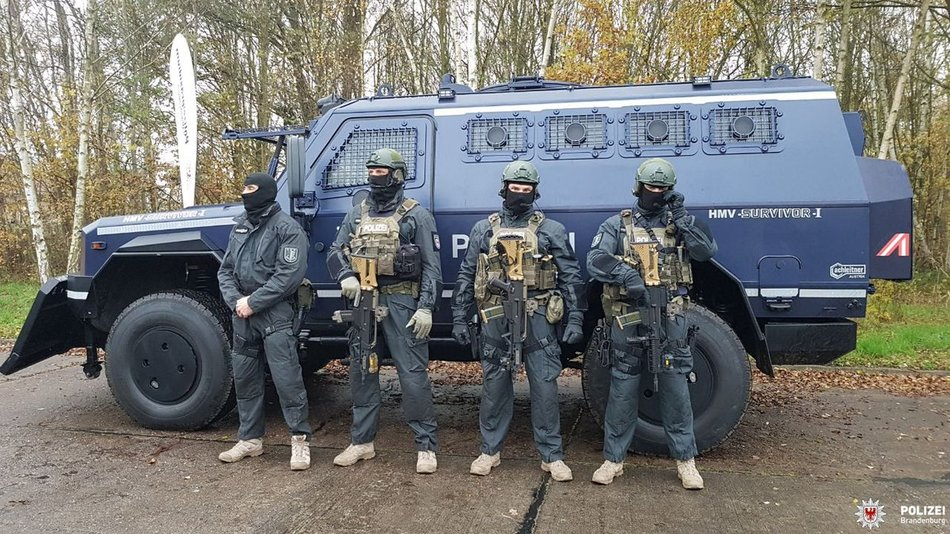
\includegraphics[width = .95\textwidth]{gfx/sek.jpg}}\\
\caption{\label{sek}{Image of the Brandenburg SEK Force. Tactical gear prioritizes safety which negatively impacts vision, mobility, and cognitive load (\cite{BradSEK}). }}
\end{figure}
\bigskip



\begin{figure}[htb]
\centering
\makebox[\textwidth]{
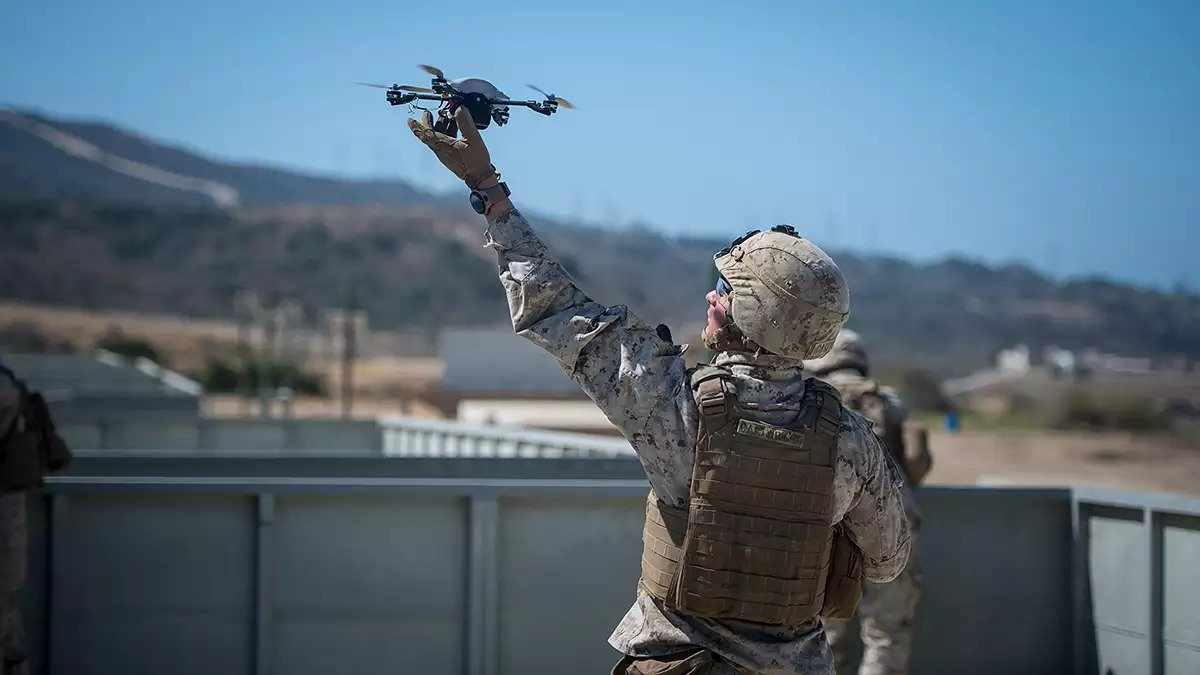
\includegraphics[width = .95\textwidth]{gfx/003.jpg}}\\
\caption{\label{usmc}{Image of USMC operative with a drone (\cite{USMC1}). }}
\end{figure}


\newpage







%\section{Motivation}
%DELETEME: This section is very important since it argues why it is necessary to take care of the problem you are addressing in your work. One way to do this is coming from a very broad view on the problem to a very detailled one. This can be done by establishing a chain of statements that refer to each other until you reach your particular problem. Doing this, you really need to take care for citing every statement. 

%DELETEME: Example for a chain: Mobile communication gets increasingly popular in the world (CITE sales on mobile communication infrastruce, mobile phones, or increasing number of mobile phones contracts). $\rightarrow$ Especially smartphones, which represent the next generation cellular phone (CITE), get more and more used for communicating not only with other people but also for connecting to the Internet for using various services (CITE). $\rightarrow$ Smartphone are comprehensive cellular phones that provide additional functionality due to their increased connection and processing capabilities (CITE). $\rightarrow$ Most smartphones offer an online application store for adding software to the devices which helps the users to customize their devices according to their needs, e.g. Android Market\footnote{\url{http://market.android.com}, visited on 05/08/2011}. $\rightarrow$ One problem about installing third-party software is that not all softwares try to help the user; $\rightarrow$ software with malicious intentions, so called malicious software (malware), can be a severe threat to smarpthone users. Some malwares delete files (EXAMPLE + CITE or footnote with URL) or even destroy devices (EXAMPLE + CITE or footnote with URL). $\rightarrow$ More and more smartphone malwares appeared in the last years (CITE). $\rightarrow$ Signature-based approaches work efficiently on known malware (CITE) but face serious drawbacks regarding unknown malware. $\rightarrow$ Oberheide et al.~\cite{oberheide:2008:cloudav} state that virus engines need an average time of 48 days until their databases get updated to be able to detect a certain unknown malware. $\rightarrow$ This in turn means that smartphone users stay unprotected for this time which can be seen as a severe threat. $\rightarrow$ Therefore, approaches are needed that are capable of detecting unknown malware for protecting the users against such threats.
%DELETEME: This example showed how one could argue that alternative approaches for malware detection is required. The length of the motivation depends on the topics handled and can of course be longer. The principle I am describing is also shown on Figure~\ref{fig:writing}

%\begin{figure}
%\centering
%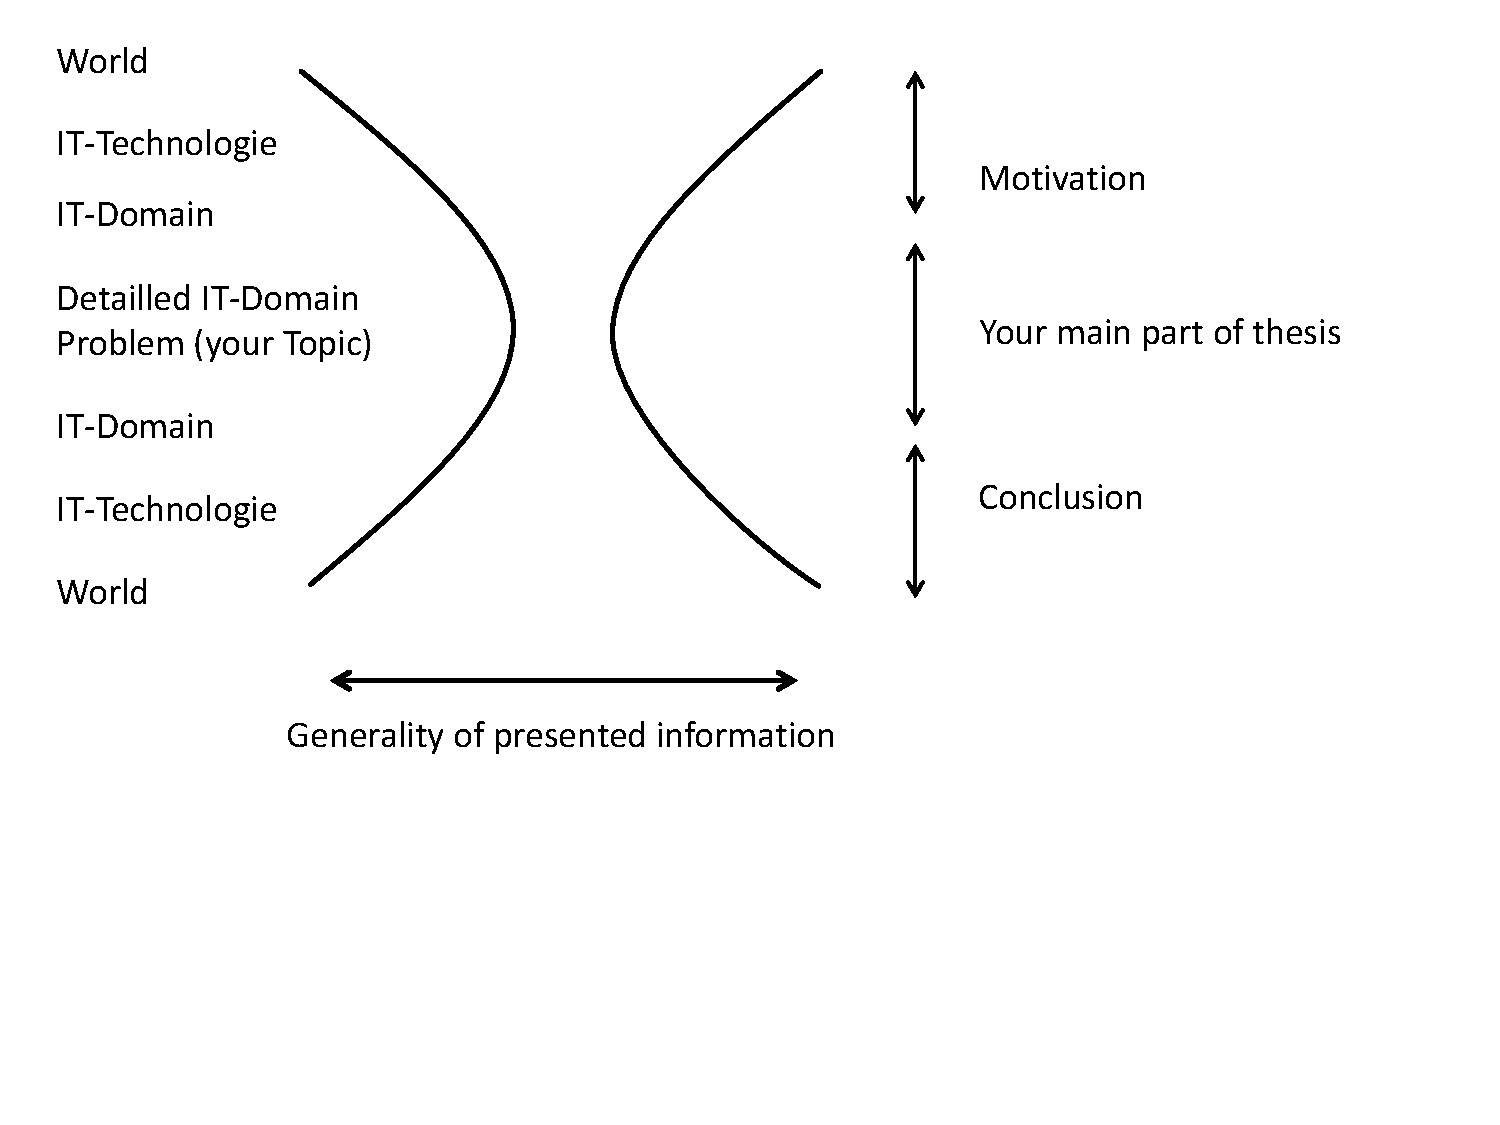
\includegraphics[width=0.9\textwidth]{template/writing}
%\caption[Information Generality]{This images illustrates how generality of information could be handled in a thesis. In your motivation you should start from a very broad view on the topic. Then you should get more precise with every statement until you reach the actual problem you are addressing. You should do vice-versa in your conclusion, starting with the problem that you addressed and getting broader until you can write about the meaning of your results to the (IT-)world.\label{fig:writing}}
%\end{figure}


%###################################################################################
%###################### Approach and Goals  ########################################
%###################################################################################
%\section{Approach and Goals}
%DELETEME: In this section, you should cleary describe your approach that you are following in order to solve the underlaying problem of your thesis. Additionally, you should clearly state the goals of your work. This will not only help you supervizor to understand what you are doing, it will also help you to be sure on which topic you should evaluate.


%###################################################################################
%###################### Structure of the Thesis ####################################
%###################################################################################
%\section{Structure of the Thesis}
%DELETEME: This section does not require eloquent writing. It is just a presentation of what you will handle in each chapter starting with Chapter~\ref{background}.

%DELETEME: Example: This thesis is structured as follows. In Chapter~\ref{background}, we discuss essential background related to the thesis topic. (SOME MORE SENTENCES). Chapter~\ref{mainone} represents a detailled analysis of the problem that will be addressed. In particular, (SOME MORE SENTENCES). In Chapter~\ref{maintwo}, our solution is presented. This solution covers ... (SOME MORE SENTENCES). Chapter~\ref{evaluation} evaluates our solution basing on our specified goals. (SOME MORE SENTENCES). In Chapter~\ref{conclusion}, we conclude. Chapter~\ref{appendices} gives additional related information on the topic of this thesis.
\chapter{Background}
%labels will help you to reference to certain images, tables, chapters, section, and so on...
\label{background}


\section{Speech Recognition}
Controlling a drone via voice commands will require several steps. First, \textit{Automatic Speech Recognition} (ASR) will need to be implemented. Since the drone will only be required to recognize and respond to a small set of words/phrases, creating a custom dictionary would be ideal (this will directly impact the memory size of the data set and can possibly result in more accurate interpretations). Next, the interpretations need to be processed and the drone's behavior needs to reflect the spoken dialog. Since the SEK is operating in dynamic and dangerous environments, this process needs to happen with high accuracy/precision and with as little delay as possible. 
\bigskip

ASR has two main approaches in implementation: either using \textit{Hidden Markov Models} (HMM) or \textit{Deep-Learning} (DL). Each implementation has a number of trade-offs and the manner of the implementation determines which approach is, in some sense, optimal. HMMs are typically easier to understand and implement (fewer parameters) at the cost of accuracy (\cite{Multimodal}). Creating HMMs for ASR requires five steps: Feature Extraction, an Acoustic Model, a Lexicon Model, a Language Model and then a Decoder (usually the Forward-Backward or Viterbi algorithms) (\cite{Stanford}). HMMs are good for problems that have a small number of states (grammar, words) and could allow for the drone to perform entirely offline (\cite{CMU1}). There is already a large library of existing solutions and implementations utilizing the CMUSphinx API (\cite{CMU-Sphinx}).
\smallskip

DL methods, usually with \textit{Convolutional Neural Networks} (CNN) or Recurrent Neural Networks (RNN) (or a combination CNN-RNN encoder/decoder \\ (\cite{Wang2016CNNRNNAU})), allow for higher accuracy in results given proper parameter tuning and a large enough dataset  (\cite{Song2015EndtoEndDN}).  DL implementations, on the other hand, will require that a network is trained with large amounts of data and the model be upload directly to the drone (or a microcontroller interface). In general, even using only an RNN will outperform an HMM (\cite{Connectionist}). More research needs to be completed prior to selecting the best candidate for ASR, as it currently seems that a DL method would be the better candidate due to its higher accuracy. The current goal is to achieve high-performance results (and an excellent demonstration). However, the focus will be to create/implement/simulate a speech recognition model that is useful for evaluating user cognitive load.
\smallskip

\textit{Text-to-Speech} and \textit{Speech-to-Text} are two methods of machine translation. Intuitively, these technologies are mappings to shift from one domain to the other. These are common in modern ASR technologies (like Alexa and Siri) for providing the user with a confirmation of audio commands. 

\section{Mixed Reality User Interface}
Once the drone can properly be given instructions via ASR, it is important that the drone is able to communicate back to the user in a meaningful manner. The main user-experience related criteria that are being pursued in this project is a 'seamless, natural integration of a drone into a mixed human-robot team.' This means that the drone needs to be able to communicate effectively (quickly, clearly, and without ambiguity). As such, there are very few approaches that would be sufficient in an environment that places a great deal of stress on the user. Haptic feedback (tactile vibrations) are likely not a good approach, as they can be easily misunderstood (and rely on the user being trained to interpret the message (\cite{Cho2003})). A speech response from the drone is also not ideal, as it requires that the user is primed for listening to the confirmation of the planned tasked (\cite{dysoncognitive}). During stress, the cognitive ability of the user will degrade (\cite{Broadbent1958-BROPAC-3}). This means that long response might be forgotten, misunderstood, or not properly heard (\cite{Engle}). Any of these events would require that the user ask the drone to repeat the flight plan. These are issues that exist even in human-human interactions, so it would be highly advantageous if a robotic system could mitigate or alleviate these issues. 
\smallskip

An alternative to tactile and audio feedback is visual feedback. This will improve the response time of the user and mitigate errors due to multi-modal bottlenecks in information processing (\cite{Sommer2001MultipleBI}). One approach would be to put LEDs on the drone that signal certain sequences of commands. Again, in this case, the operator needs to be trained to interpret these responses from the drone. Furthermore, once the drone is out of the line-of-sight, the drone will not be able to effectively communicate with visual commands. Therefore, a UI within a Mixed Reality device (i.e., HoloLens) can also be utilized. The UI can be designed in a mixed-reality format that displays, with written words or intuitive icons, the flight/task plan of the drone. It is hypothesized that this will mitigate the forgetfulness of the user due to the high cognitive load. The UI could be designed in a manner that will not impede the vision of the user. This allows the user to maintain situational awareness and analyze the feedback when deemed safe. Regardless, both audio and visual solutions need to be approached as often times theory and reality do not match in real-world implementations. 

%%\subsection{Gesture Recognition and Integration}
%To approach RQ3, the previous work taken place at the Distribution Artificial Intelligence Laboratory (DAI-Labor) would be extended \cite{Montebaur}. The general idea is to allow the drone to allow for multi-modal inputs (speech and/or visual). The motivation for this is that the more critical missions (espionage, infiltration) require users to be silent (covert operations). Therefore, speech-related commands need to be minimized. However, the noise the drone emits is still an issue. Therefore, it might be beneficial to allow the drone to receive flight/task plans prior to motor activation. 
\smallskip

%Furthermore, it might be the case that only small, manual movements are desired for the drone. A use-case scenario for this would be as follows: a drone had completed a flight plan to enter into a specific room but has not located any targets and is idling on location. The operator, using a mixed-reality or video-streaming device, has access to the feed of the drone. The human operator believes that he sees something that the drone does not and wants to make small adjustments to the drone's location or heading. This could be done with manual operation using the PeriSense controller. (Perhaps the user wants to view specific infrastructure damage, find a target hiding from the drone, or analyze other environmental hazards that the drone has not yet been taught how to observe). 

\section{Robot Behavior Planning}

In mixed human-robot teams, predictable and reliable agent behavior is crucial.  \cite{hrabia1} have created a framework that allows for multi-agent environments with adjustable parameters such as pose, distance, and movements. When considering having a drone (or another robot agent) adjust behavior depending on both the user and the environment (both dynamic), a flexible approach to decision making and planning is desired. This would allow for the drone to change is behavior in real-time without compromising the mobility/visibility of the operator or negatively interacting with the environment (i.e., crashing into a wall). 
\smallskip

The \textit{ROS Hybrid Behavior Planner} (RHBP) seeks to meet these requirements with a hybrid reactive-adaptive behavior-based planner. This is a major improvement over traditional approaches (conditional statements) that do not have any weights, probabilistic characteristics or allow for (potential) reinforcement learning models. 

\section{Cognitive Load Theory and Testing}
Many different tests have been created to evaluate the cognitive performance of individuals during various conditions. \textit{Situational Awareness} is limited by available resources in memory capacity and computation during decision-making (\cite{Endsley}). When resources are limited or have been depleted, users begin to make errors in accuracy or decision making as a result. Cognitive load (and SA) can be evaluated with two types of tests: qualitative and quantitative. A common qualitative test is the NASA Task Load Index (NASA-TXL) which allows users to access their \textit{perceived} stress and workload levels while completing other tasks. Another traditional test is based on Cognitive Load Theory (CLT) in which subjects report their perceived performance after tasks are given for problem-solving or spit-attention (\cite{Chandler}).


For qualitative experiments, attention, working memory, and response time are common metrics. The \textit{Operation Span Task} (OSPAN) is used to measure the \textit{Working Memory} capacity of users (\cite{ospan2}). This is completed by giving the user an item to remember and then interjecting with random simple mathematics problems, after which they are asked to recall the item. In the case of drone operations, a set of directions could be provided as the `item.' The \textit{Attentional Blink} test is used to measure the response time and accuracy of a user when two items are displayed for brief periods of time with a short (variable) delay between objects (\cite{Nieuwenstein}). NASA has employed the \textit{Psychomotor Vigilance Task} to measure the cognitive performance of astronauts during space missions (NASA Extreme Environment Mission Operation NEEMO (\cite{nasa2})) and aboard the International Space Station. This test measures the response time for the user to press a keyboard after an image has been displayed on a screen (faster is better). 
%%%%%%%%%%%%%%%%%%%%%%%%%%%%%%%%%%%%%%%%%%%%%%%%%%%%%%%%%%%
%DELETEME: This chapter will cover all of your background information and related work. Background and related work are directly related to your thesis. Please do not place irrelevant content here which is a common mistake. Citing will be handled in the appendices.

%DELETEME: Background represents underlaying knowledge that is required to understand your work. The expected knowledge level of your readers can be set to the one of a bachelor or master student who just finished his studies (depending on what kind of thesis you are writing). This means that you do not need to describe how computers work, unless your thesis topic is about this. Everything that an avarage alumni from your field of studies should now does not need to be described. It turn, background information that is very complex and content-wise very near to you problem, can be placed in the main parts. Everyting else should be written here. Note: it is important to connect each presented topic to your thesis. E.g. if you present the ISO/OSI layer model you should also write that this is needed to understand the protocols you plan to develop in the main parts.

%DELETEME: Related work respresents results from work that handled the same or a similar problem that you are addressing. This work might have used a different approach or might not have been that successful. Finding a paper / work that solved your problem in the same way you were planning to do is not good and you should contact your supervizor for solving this issue. Again, each paper / work has to be connected to your approach: other papers might have not chosen an optimal solution; they might not have been taking care of essential aspects; they might have chosen a different approach and you believe, yours will work better ...

%###################################################################################
%###################### Topic A             ########################################
%###################################################################################
%\section{Topic 1}

%###################################################################################
%###################### Topic B             ########################################
%###################################################################################
%\section{Topic 2}

%###################################################################################
%###################### Topic C             ########################################
%###################################################################################
%\section{Topic 3}
\chapter{My First Main Part}
\label{mainone}
%DELETEME: In this chapter you start addressing your actual problem. Therefore, it makes often sense to make a detailed problem analysis first (if not done in introduction). You should be sure about what to do and how. As writtin in the background part, it might also make sense to include complex background information or papers you are basing on in this analysis. If you are solving a software problem, you should follow the state of the art of software development which basically includes: problem analysis, design, implementation, testing, and deployment. Maintenance is often also described but I believe this will not be required for most theses. Code should be placed in the appendix unless it is solving an essential aspect of your work.

\section{Objectives}

Note: each RQ will be approached and completed with the mindset that this is not a final, shippable product, i.e., this is a prototype/mock-up. In reality, the foundation and framework need to be available in the form of a robust 'proof-of-concept' that can be adaptable for specific needs of the stakeholders that follow (e.g., the SEK will likely want to change specific details as well as future researchers within the DAI-Labor). 
\smallskip

Each research question will be broken down into work packages. Each implementation will be given clear objectives and criteria for evaluation. Some work packages will have a slight overlap related to tuning, implementation, and iterative design. The end results are intended for the interoperability between distributed systems, applicable to many projects. 
\smallskip

\subsection{RQ1: Human-Robot Communication}
\noindent RQ1: How should the drone send confirmations to the operator to minimize ambiguity, human errors, and temporal descrepancies?
\smallskip

After viewing the field demonstration and discussion with the SEK, it is evident controlling the drone via voice commands is preferred. The SEK operatives primarily utilize speech (through headsets) for communication (local and global). While gestures, positioning, and other non-verbal communication methods are employed (i.e., patting and tapping) this are based on proximity (locality) and the situation. Furthermore, as local communication is based on quick confirmations, it does not appear to impact the overall goal. As such, the drone will still have its core mission criteria that are independent of these non-verbal interactions. 
\smallskip

Once the drone has received its orders, it should begin to complete its tasks. However, it is currently not clear how the drone will communicate with the operator that it has correctly interpreted the task. Consider the following task given to a drone: 'go forward to an open doorway, enter the room, scan the area, proceed into any additional room on the right side.' It is possible that the drone correctly begins its task and enters the first room but did not properly interpret the sequence afterward. If the drone is able to confirm the sequence with the operator, proper navigation can be ensured (at least on the command level). Furthermore, it would be ideal to give a drone a sequence of commands with a 'wait' feature, i.e., \texttt{sleep()}. The operator could properly confirm the sequence, make any necessary changes, and then send an 'engage' command. The drone should also be able to send confirmations once each individual command has been completed (like a check-list) if desired. 
\smallskip

In designing \textit{Natural User Interfaces} (NUIs), research has shown that gesture-based interfaces are less natural for communication. Due to the high criticality of missions and adherence to safety, any additional ambiguity related to NUIs would impact mission performance. Audial and visual interfaces can decrease ambiguity if properly designed. The first logical step is to determine which of these two interfaces are preferred prior to detailed implementation. Therefore, a user study needs to be conducted evaluating preference, subjective load, and qualitative factors. 



\subsection{RQ2: Operator Cognitive Load}
\noindent RQ2: What are the negative effects (response time delay, accuracy, situational awareness) on the operator's cognitive load during operation?
\smallskip

Automatic Speech Recognition (ASR) models are not perfect. The middleware might not properly understand the commands of the user which greatly impacts the mission's objectives due to a loss of time for correction and operator frustration/distraction. A user study will be needed in which the user completes some simple tasks simultaneously as validating the drone's confirmation. The concept here is that a drone could report to the operator incorrect information which could lead to mission failure and/or compromise the operator/plan. For quantitative evaluation, several tests from the cognitive science field have been employed to measure \textit{Working Memory} (WM) capacity (is the operator able to properly remember the sent commands when under pressure?) and \textit{Response Time} during events requiring a high cognitive load and split attention. The results and analysis will infer user's situational awareness and confirmation accuracy. The user could be asked to give commands to the drone and listen for the confirmation while taking the test. Quantitative results would be compared between a baseline (test only), test while receiving audial confirmations (headset), and tests while receiving visual confirmation (AR).
\smallskip

\section{Proposed Solution}

Based on the previous sections, the goal is to enable a drone to accept user commands, accurately follow the commands, and send a confirmation to the user (for review). Prior to selecting the form in which the drone should send confirmations, qualitative (user preference) and quantitative (reaction times, accuracy of memory) need to be derived from user study results. The simulation environment will be based on the previous work at DAI-Labor (\cite{hrabia1}). A custom library/dictionary will be created for ASR and validated in ROS. ROS will then communicate these commands to the drone (SST) and the drone's behavior should follow correctly. It is planned to create a UI for visual representations of the confirmation (a text-based or icon-based visualization) depending on the Mixed-Reality device (i.e., Unity 3D for HoloLens). 


\subsection{Milestone I}
%RQ1 will have several distinct phases. First, a library/dictionary for \textit{Automated Speech Recognition} (ASR) must be created/utilized. Secondly, the library must be properly processed and published in ROS. Third, interfacing and validation in real-time (or pre-recorded .WAV files) will be completed on a drone in the simulator. Then, if access is available, demonstrating the simulation results on a live drone (much like the previous InLaSeD work \cite{Montebaur}). 

RQ1 and RQ2 will be approached simultaneously. The first aspect is to implement a library/dictionary for \textit{Automated Speech Recognition} (ASR) that can allow for commands to be sent to a drone (either simulated or actually sent to a drone via ROS). Next, a Speech-to-Text (STT) library could be designed for machine translation into ROS (ideal of verification of commands). In the physical implementation of a drone, the STT commands would be sent to the robot. For cognitive evaluation alone, it might be better to focus on a Text-to-Speech (TTS) model. Utilizing a terminal, TTS commands could be manually typed and sent to the user's device to evaluate their hit/miss rate for confirming the drone's response. This would mitigate any errors that would be caused by utilizing ASR (control variable). TTS commands would be sent to the user's headset during a cognitive test. For an MR solution, STT would allow for commands to be translated and sent to the device's UI in the form of words or icons that represent words (i.e., a right arrow for `right'). 
\smallskip

It is intended to use the NASA-TXL (or similar) for measuring perceived cognitive load while asking users to make a preference for receiving audial or visual confirmations. For quantitative tasks, it is intended to use the Inquisit Laboratory program with the PVT test. Both tests are regularly used by NASA to evaluate astronauts during space missions, furthermore, NASA quotes: "The PVT Self Test has wide application to any group that must operate remotely at high levels of alertness, such as first responders, Homeland Security personnel, flight crews, special military operations, police, and firefighters (\cite{nasa1})." This makes the test ideal in evaluating subjects for high cognitive load tasks. The current plan is to evaluate three use cases for the test: one without any drone commands (baseline), one with audial drone confirmations, and one with visual drone confirmations. The goal is to have the users complete the tasks of the PVT while measuring their response times and accuracy (automatic with Inquisit Laboratory (\cite{Millisecond})) and documenting their accuracy for confirming correct drone command sequences (hit). 

\subsection{Milestone II}
After qualitative and quantitative results have been analyzed and weighed, a virtual implementation can be thoroughly constructed in ROS (with an RHBP model). The task will be to ensure that drone behavior matches the input commands and the output is properly sent to the user's device. Additionally, the drone will operate within the selected range/bounds based on the operational criteria based on SEK operatives, as well as an interoperable model that can be used for general projects (a distributed model). Finally, once the behavior has been validated and verified in ROS, it is intended to provide a live demonstration with the drone responding to the user commands, following intended behavior, and reporting back to the user's device. 
\smallskip

%\subsection{Milestone II}
%RQ3 will also require user testing. The goal will be to operate a drone at varying distances, heights, and relative angles from the user. For this, a custom test will be made in which the users describe their preferences. In the ranges that have the most overlap, a model can be created in the RHBP. 
%\smallskip

%\subsection{Milestone III}
%RQ4 will require careful implementations for drone behavior. The goal is to take the results of RQ3 and have a drone operate within the selected range/bounds along with additional operational criteria based on SEK operatives. Ideally, an artificial human agent will be created, along with an environment that has realistic features (narrow hallways, staircases, objects, etc.). The goal is to have the drone perform as a useful teammate that does not impede the mission plan, safety, or cognitive load of the SEK operative. Based on the results here, it can be decided on \textit{how} to add sensors to the drone to properly understand spatial relations to the operator. 
%\smallskip

\subsection{Project Management}
Typical project management aspects will also follow. A GitLab account will be created via TU Berlin and Scrum-style weekly meetings will be conducted with Christopher-Eyk Hrabia. This will help to ensure timeliness and proper communication. Deviations are likely to happen (i.e., switching from one framework to another due to compatibility or performance issues) but this will be mitigated as much as possible with proper literature review and stand-alone implementations.


\section{Work Packages}
The project will be broken down into several work packages. Figure \ref{gannt} gives the timeline for task completion. This section proposes some of the current approaches and architectures.


\subsection{Research}

Research has been conducted, thus far, by first evaluating the goal of the project. This has made the approach easier by evaluating how other researchers have approached this issue (from classical methods to state-of-the-art). Next, it was critical to ensure the alignment of the needs of the SEK. This pruned a lot of approaches and methods. However, more iterations within the research cycle need to continue in order to meet the high-performance metrics while maintaining feasibility. 


\subsection{Implementation Process}


It is planned to make a library based on the commands that SEK operatives would use during operations. Such words might include 'forward', 'right', and 'stop'. Furthermore, temporal and spatial commands would be ideal ('forward for five seconds', 'left two meters'). However, spatial commands need a proper translation from the user's perspective to the drone's perspective. If possible (and in existence) it would be good to allow for a command that switches to autonomous behavior ('exploration/scan mode'). This will depend on what the drone is already capable of (or added as part of this project by pruning another research question). Each utterance (word) will need to be recorded at least 200 times. This will help provide enough data for a DL implementation with TensorFlow (see below). If this is insufficient, more recordings will be created. For HMM models, it is not clear how much training data is needed currently. The resulting model can be tested (if required) with users but it might be better to treat the proposed user testing with a `simulated' environment (i.e., manually sending congruent/incongruent command sequences via TTS or text-based inputs). 
\smallskip


Until now, a large amount of time was spent to ensure that the project was feasible. ROS is intended to be the core middleware for program communication. Many considerations were given based on the (real) environment that the drone would operate in. For example, Cloud computing for ASR allows for the highest accuracy using Google's STT framework (\cite{Google}). However, Cloud interfaces might not be plausible and soldiers might not be in an environment that can directly interact with the Cloud.
\smallskip

Currently, the plan is to create an independent library and either utilize DL via TensorFlow (\cite{TensorFlow}) based on Small-footprint Keyword Spotting \\ (\cite{keyword}) or use a HMM model with PocketSphinx and a custom dictionary. TensorFlow can easily integrate with ROS and is relatively easy to adjust. Furthermore, the TensorFlow implementation allows for continuous speech input and the trained models can be exported to Android (good for in-person demonstrations). Finally, results can be visualized using TensorBoard, an aesthetic and informative tool. In terms of an HMM approach, many researchers have used CMU-Sphinx (PocketSphinx) for ASR. Achieving the highest accuracy possible is desired, so the final implementation may require the DL/TensorFlow approach as HMM can have variable accuracy as the end result (which is undesirable for safety-critical missions) (\cite{Amazigh}), (\cite{Covariance}). 
\smallskip

In the event there are issues with the speech recognition in ROS, it can be bypassed and completed in Unity 3D (worst-case scenario) (\cite{Unity}). Unity can act as middleware, though it often behaves slower. This would only be in the case of a demonstration that was also utilizing the HoloLens (as is done by Siemens (\cite{Siemens})). However, a HoloLens might not be available and another device (which will likely be lighter and better for cognitive load) will need to be used. If it does not have an interface with Unity, another solution will be employed. Another option is to directly employ the Google Cloud Speech API in ROS. Again, based on the assumptions I have proposed, this is not ideal and would be left only for the sake of demonstration (i.e., for the SEK with a very constrained deadline) (\cite{Google2}). 
\smallskip

The UI will be created using Unity 3D (HoloLens) or similar software (third-party AR/MR device). This allows for some visualizations and initial feedback even without having a device on hand. In fact, it could be that this lays the framework for implementation (as a proof-of-concept) in the event that a HoloLens is unobtainable.



\chapter{My Second Main Part}
\label{maintwo}
\chapter{Evaluation}
\label{evaluation}
DELETEME: The evaluation chapter is one of the most important chapters of your work. Here, you will prove usability/efficiency of your approach by presenting and interpreting your results. You should discuss your results and interprete them, if possible. Drawing conclusions on the results will be one important point that your estimators will refer to when grading your work.

%###################################################################################
%###################### Results             ########################################
%###################################################################################
\section{Results}
\label{results}

%###################################################################################
%###################### Discussions         ########################################
%###################################################################################
\section{Discussions}
\label{discussions}
\chapter{Conclusion and Future Work}
\label{conclusion}
%#############################################################
%###################### Summary   ############################
%#############################################################
\section{Summary}
DELETEME: put a plain summary of your work here. Summaries should be made of each Chapter beginning with Chapter~2 and ending with you evaluation. Just write down what you did and describe the corresponding results without reflecting on them.

%#############################################################
%###################### Conclusion ###########################
%#############################################################
\section{Conclusion}
DELETEME: do not summarize here. Reflect on the results that you have achieved. What might be the reasons and meanings of these? Did you make improvements in comparison to the state of the art? What are the good points about your results and work? What are the drawbacks? 

%#############################################################
%###################### Future Work ##########################
%#############################################################
\section{Future Work}
DELETEME: Regarding your results - which problems did you not solve? Which questions are still open? Which new questions arised? How should someone / would you continue working in your thesis field basing on your results?

%__________________________End_of_Thesis______________________________________________
\cleardoublepage
\addcontentsline{toc}{chapter}{Bibliography}
%harvard citations style, please uncomment harvard package in the usepackage area
%\bibliographystyle{agsm}
%remove the following line when using harvard style citation
%\bibliographystyle{plainnat}
\bibliographystyle{apalike}
%specify bibtex file here
\bibliography{input/mybib}
%add appendix to TOC
\addcontentsline{toc}{chapter}{Appendices}
\chapter*{Appendices}
\label{appendices}
DELETEME: everything that does not fit into your work, e.g. a 5 page table that breaks the reading flow, should be placed here

%###################################################################################
%###################### Appendix A          ########################################
%###################################################################################
%uncomment, if desired
%\newpage
\addcontentsline{toc}{section}{Appendix A: Abbreviations}
\section*{Appendix A: Abbreviations}
\begin{center}
\begin{tabular}{ll}
\textbf{ASR}	&	Automatic Speech Recognition (Automatische Spracherkennung)\\
\textbf{CNN}	&	Convolutional Neural Network \\
\textbf{DL}		&	Deep-Learning (Tiefes Lernen)\\
\textbf{HMM}	&	Hidden Markov Model (verdecktes Markowmodell)\\
\textbf{NEEMO}	&	NASA Extreme Environment Mission Operation\\
\textbf{OSPAN}	&	Operation Span Task (Operationsspanne Aufgabe)\\
\textbf{RNN}	&	Recurrent Neural Network (Rekurrentes neuronales Netz)\\
\textbf{LED}	&	Light Emitting Diode (lichtemittierende Diode)\\
\textbf{LSB}	&	Least Significant Bit\\
\textbf{MD5}	& Message Digest (Kryptographisches Fingerabdruckverfahren)\\
\textbf{MPEG}	&	Moving Picture Experts Group (Video- einschließlich Audiokompression)\\
\textbf{MP3}	&	MPEG-1 Audio Layer 3 (Audiokompressionformat)\\
\textbf{PACS}	&	Picture Archiving and Communication Systems\\
\textbf{PNG}	&	Portable Network Graphics (Grafikformat)\\
\textbf{RSA}	&	Rivest, Shamir, Adleman (asymmetrisches Verschlüsselungsverfahren)\\
\textbf{SHA1}	&	Security Hash Algorithm (Kryptographisches Fingerabdruckverfahren)\\
\textbf{WAV}	&	Waveform Audio Format (Audiokompressionsformat von Microsoft)\\
%\textbf{abk}	&	erklärung\\
%\textbf{abk}	&	erklärung\\
%\textbf{abk}	&	erklärung\\
%\textbf{abk}	&	erklärung\\
%\textbf{abk}	&	erklärung\\
%\textbf{abk}	&	erklärung\\
%\textbf{abk}	&	erklärung\\
%\textbf{abk}	&	erklärung\\
%\textbf{abk}	&	erklärung\\
%\textbf{abk}	&	erklärung\\
%\textbf{abk}	&	erklärung\\
%\textbf{abk}	&	erklärung\\
%\textbf{abk}	&	erklärung\\
\end{tabular}
\end{center}

%###################################################################################
%###################### Appendix B          ########################################
%###################################################################################
\newpage
%change this
\addcontentsline{toc}{section}{Appendix B: {\LaTeX} Help}
\section*{Appendix B: {\LaTeX} Help}
%remove this
%###################################################################################
%###################### HowTo               ########################################
%###################################################################################
\subsection*{How to Use This Template}
\begin{itemize}
\item Remove all of my text which is mostly labeled with DELETEME
\item Change the information in the 00a\_title\_page.tex file
\item Use the information written in this section
\item Ask you supervizor to help you
\item If I am not your supervizor and noone else can help you, write me an email (aubrey.schmidt@dai-labor.de)
\end{itemize}

%###################################################################################
%###################### Citations           ########################################
%###################################################################################
\subsection*{Citations}
Citing is one of the essential points you need to do in you thesis. Statements not basing on results of your own research\footnote{in what ever context} not being cited represent a breach on the rules of scientific working. Therefore, you every statement needs to be cited basing on information that other people can cross-check. A common way of citing in technical papers is: 
\begin{itemize}
\item Oberheide et al.~\cite{oberheide:2008:cloudav} state that the average time for an anti-virus enginge to be updated with a signature to detect an unknown threat is 48 days.
\end{itemize}
Note: et al. is used when the paper was written by more than two people. Check the code of this section to learn how to cite from a technical perspective.

Note: you can change the citation style in the \texttt{thesis.tex} file, e.g. to harvard style citations. Instructions on this can also be found in this file.

You should not cite anything that can be changed, e.g. it is not that good citing web pages since they might get updated changing the cited content. There are no clear quality measures on citing sources but aubrey believes that the following list is true for several cases, starting with highest quality:
\begin{enumerate}
\item Journal article or book
\item Conference paper
\item Workshop paper
\item Technical report
\item Master thesis
\item Bachelor thesis
\item General Web reference
\end{enumerate}
There might be workshop papers that have a higher quality than some journal papers. Therefore this list only gives you a hint on possible quality measures. Another measure can be whether a paper was indexed by ACM/IEEE, although this is not a strong indicator.

%###################################################################################
%###################### Papers             ########################################
%###################################################################################
\subsection*{Finding and Handling Citation Sources}
Following ressources are required for finding and handling articles, books, papers and sources.
\begin{itemize}
\item your primary resource will be \url{http://scholar.google.com}
\item \url{http://www.google.com} might also be used
\item \url{wikipedia.com} can be a good start for finding relevant papers on your topic
\item you should download and install JabRef or a similar tool \url{http://jabref.sourceforge.net/}
\item you should point JabRef to the mybib.bib file
\item you should immediately enter a relevant paper to JabRef, additionally, you should write a short summary on it; else, you will do this work at least twice.
\end{itemize}

%###################################################################################
%###################### General             ########################################
%###################################################################################
\subsection*{General Advices}
\begin{itemize}
\item Do not take care of design, \LaTeX will do this for you. If you still feel that you need to take care of this, do this when you have finished writing, else you will end up in a lot of double and triple work.
\item \LaTeX will do exactly that you will tell it to do. If you have problems with this, go for google or ask you supervizor
\item use labels in order to be able to reference to chapters, section, subsections, figures, tables, etc. ...
\end{itemize}

%###################################################################################
%###################### Commands            ########################################
%###################################################################################
\subsection*{General Commands}
\begin{itemize}
\item check \url{http://en.wikibooks.org/wiki/LaTeX}
\item check \url{http://www.uni-giessen.de/hrz/tex/cookbook/cookbook.html} German
\end{itemize}
Please also check the following source~\cite{latexcookbook2007}.

%###################################################################################
%###################### Code                ########################################
%###################################################################################
\newpage
\subsection*{Code}
This section shows you how to get your code into a \LaTeX document. See code for options.
\lstinputlisting[language=JAVA,xleftmargin=8mm,]{help/Example.java}


\lstset{ %
language=Java,   	             % the language of the code
numbers=left,
basicstyle=\scriptsize,       % the size of the fonts that are used for the code
numbers=left,                   % where to put the line-numbers
numberstyle=\scriptsize,      % the size of the fonts that are used for the line-numbers
stepnumber=1,                   % the step between two line-numbers. If it's 1, each line 
                                % will be numbered
numbersep=5pt,                  % how far the line-numbers are from the code
backgroundcolor=\color{white},  % choose the background color. You must add \usepackage{color}
showspaces=false,               % show spaces adding particular underscores
showstringspaces=false,         % underline spaces within strings
showtabs=false,                 % show tabs within strings adding particular underscores
frame=single,                   % adds a frame around the code
tabsize=2,                      % sets default tabsize to 2 spaces
captionpos=b,                   % sets the caption-position to bottom
breaklines=true,                % sets automatic line breaking
breakatwhitespace=false,        % sets if automatic breaks should only happen at whitespace
title=\lstname,                 % show the filename of files included with \lstinputlisting;
                                % also try caption instead of title
xleftmargin=8mm,
framexleftmargin=4mm,           
escapeinside={\%*}{*)},         % if you want to add a comment within your code
morekeywords={*,...}            % if you want to add more keywords to the set
}
\begin{lstlisting}[float=h, caption=Example code is presented here, label=list:code, frame=single]
class Beispiel{

	public static void main(String args[]){
	
		System.out.println("Hello World");
		
	}
	
}
\end{lstlisting}

%###################################################################################
%###################### Figures             ########################################
%###################################################################################
\newpage
\subsection*{Figures}
This section describes how to include images to your document. Information was taken from \url{http://en.wikibooks.org/wiki/LaTeX/Floats,_Figures_and_Captions}, visited on 05/08/2011. Please make sure to use original vector graphics as basis since image quality might be used as weak indicator for thesis quality. For this, try to find find files in \texttt{.SVG} or \texttt{.PDF} format. Exporting a \texttt{.PNG} or \texttt{.JPG} to \texttt{.PDF} will not work since data was already lost while exporting it to these formats. This is the case for most Web graphics. Wikipedia startet entering most in images in \texttt{.SVG} which easily can be transformed to \texttt{.PDF}, but please do not forget proper citations.

%use a modifier to decide where you desire Latex should put the image: (h)ere, (t)op, (b)ottom, or nothing more than that image on a (p)age
\begin{figure}[h]%[htbp]
%this will center your image
\centering
%this will include your image
\includegraphics[width=0.15\textwidth]{template/TUBerlin_Logo_rot_hell}
%this is the caption + label. the label will not be printed in the caption. Moving the label out of the caption can result in problems.
\caption[Including an Image]{Including an image; in this case a PDF. Please note that the caption is placed below the image.\label{fig:help1}}
\end{figure}

\begin{figure}[h]
%this will center your image
\centering
%this will include your image

\includegraphics[width=0.25\textwidth]{template/aot_logo}
%this is the caption + label. the label will not be printed in the caption. Moving the label out of the caption can result in problems.
\caption[Short caption for list of figures]{See code for caption options: this is a long caption which is printed in the Text. Additionally, image size was increased\label{fig:help2}}
\end{figure}


\begin{figure}[h]
  \centering
  \subfloat[Small]{\label{fig:tub1}\includegraphics[width=0.1\textwidth]{template/TUBerlin_Logo_rot_hell}}                
  \subfloat[Large]{\label{fig:tub2}\includegraphics[width=0.3\textwidth]{template/TUBerlin_Logo_rot_hell}}
  \subfloat[Medium]{\label{fig:tub3}\hspace{2cm}\includegraphics[width=0.2\textwidth]{template/TUBerlin_Logo_rot_hell}}
  \caption[Placing images side by side]{Placing images side by side using the subfig package. Space between the images can be adjusted.\label{fig:tuball}}
\end{figure}


%###################################################################################
%###################### Tables              ########################################
%###################################################################################
\newpage
\subsection*{Tables}
Here, you will find some example tables.The tables were taken from \url{http://en.wikibooks.org/wiki/LaTeX/Tables}, visited on 05/08/2011. Table environment was added plus caption and label. For code, check \url{__help/latex_hinweise.tex}.

\begin{table}[h]
\caption{Simple table using vertical lines. Note that the caption is always above the table! Please check code for finding the right place for the table label.\label{tab:help1}}
\centering
  \begin{tabular}{ l | c || r | }
    \hline
    1 & 2 & 3 \\ \hline
    4 & 5 & 6 \\ \hline
    7 & 8 & 9 \\
    \hline
  \end{tabular}
\end{table}

\begin{table}[h]
\caption{Table using vertical and horizontal lines\label{tab:help2}}
\centering
\begin{tabular}{|r|l|}
  \hline
  7C0 & hexadecimal \\
  3700 & octal \\ \cline{2-2}
  11111000000 & binary \\
  \hline \hline
  1984 & decimal \\
  \hline
\end{tabular}
\end{table}

\begin{table}[h]
\caption{Table with column width specification on last column\label{tab:help3}}
\centering
    \begin{tabular}{ | l | l | l | p{5cm} |}
    \hline
    Day & Min Temp & Max Temp & Summary \\ \hline
    Monday & 11C & 22C & A clear day with lots of sunshine.  
    However, the strong breeze will bring down the temperatures. \\ \hline
    Tuesday & 9C & 19C & Cloudy with rain, across many northern regions. Clear spells
    across most of Scotland and Northern Ireland,
    but rain reaching the far northwest. \\
    \hline
    \end{tabular}
\end{table}

\begin{table}[h]
\caption{Table using multi-column and multirow\label{tab:help4}}
\centering
\begin{tabular}{|l|l|l|}
\hline
\multicolumn{3}{|c|}{Team sheet} \\
\hline
Goalkeeper & GK & Paul Robinson \\ \hline
\multirow{4}{*}{Defenders} & LB & Lucus Radebe \\
 & DC & Michael Duberry \\
 & DC & Dominic Matteo \\
 & RB & Didier Domi \\ \hline
\multirow{3}{*}{Midfielders} & MC & David Batty \\
 & MC & Eirik Bakke \\
 & MC & Jody Morris \\ \hline
Forward & FW & Jamie McMaster \\ \hline
\multirow{2}{*}{Strikers} & ST & Alan Smith \\
 & ST & Mark Viduka \\
\hline
\end{tabular}
\end{table}







\end{document}
